\section{GİRİŞ}

Radar (Radio Detection and Ranging) sistemleri, çevrede bulunan nesnelerin algılanması, konumlandırılması ve izlenmesi amacıyla kullanılan önemli algılama sistemleridir. Gerçek radar sistemleri elektromanyetik dalga gönderme, yansıyan sinyali alma ve bu sinyal üzerinden mesafe, yön ve hız bilgisi çıkarma prensibine dayanır. Savunma sanayisi, hava trafik kontrolü, otonom araçlar, robotik sistemler ve endüstriyel otomasyon gibi birçok alanda radar benzeri algılama sistemleri kritik görevler üstlenmektedir.

Bu çalışmada geliştirilen sistem, gerçek bir RF radar sistemi değildir; ancak radar sistemlerinin temel tarama ve hedef gösterim mantığını eğitim amaçlı olarak modelleyen gömülü bir prototiptir. Arduino Uno mikrodenetleyici kartı temel alınarak oluşturulan sistemde, çevre taraması pan-tilt mekanizması ile gerçekleştirilmekte, mesafe algılama Sharp GP2Y0A02YK0F kızılötesi sensör üzerinden yapılmaktadır. Elde edilen ölçümler hem yerel LCD ekranda gösterilmekte hem de web arayüzüne aktarılarak polar radar ekranı üzerinde görselleştirilmektedir.

Projenin temel motivasyonu, gömülü sistemler dersinde yalnızca sensör okuma veya servo kontrolü yapan basit bir uygulama yerine; donanım, yazılım, haberleşme, veri kaydı ve kullanıcı arayüzünü aynı mimaride birleştiren daha kapsamlı bir sistem geliştirmektir. Bu nedenle projede servo motor kontrolü, analog sensör okuma, I2C haberleşmesi, SPI tabanlı SD kart kullanımı, MPU6050 üzerinden hareket/titreşim takibi, JSON tabanlı seri veri aktarımı ve Web Serial API ile tarayıcı tabanlı gerçek zamanlı görselleştirme birlikte ele alınmıştır.

Sistemin genel mimarisi Şekil~\ref{fig:blok_sema}'de, fiziksel bağlantı yapısı ise Şekil~\ref{fig:tum_sistem}'de verilmiştir.

\begin{figure}[H]
\centering
    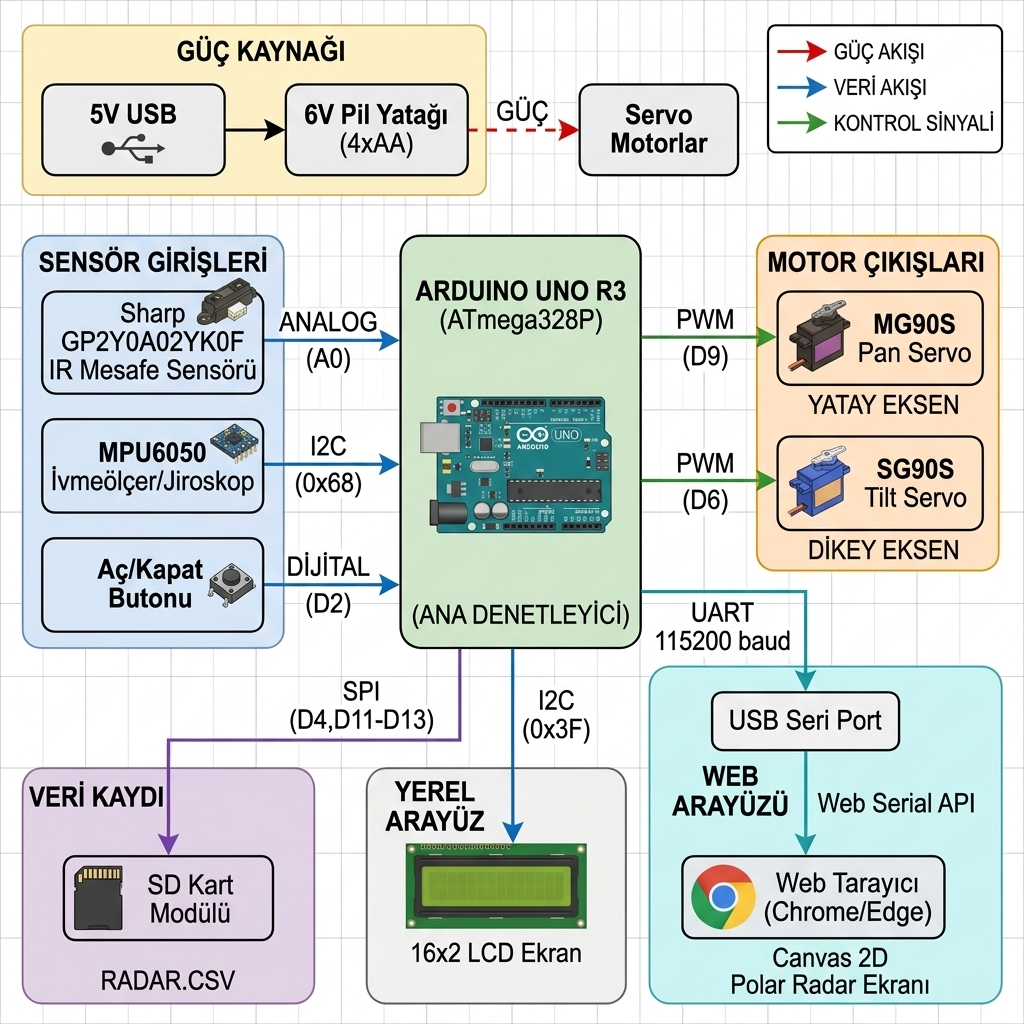
\includegraphics[width=0.84\textwidth]{sistem_blok_semasi.png}
    \caption{Pan-Tilt IR Radar sistemi blok şeması}
    \label{fig:blok_sema}
\end{figure}

\begin{figure}[H]
\centering
    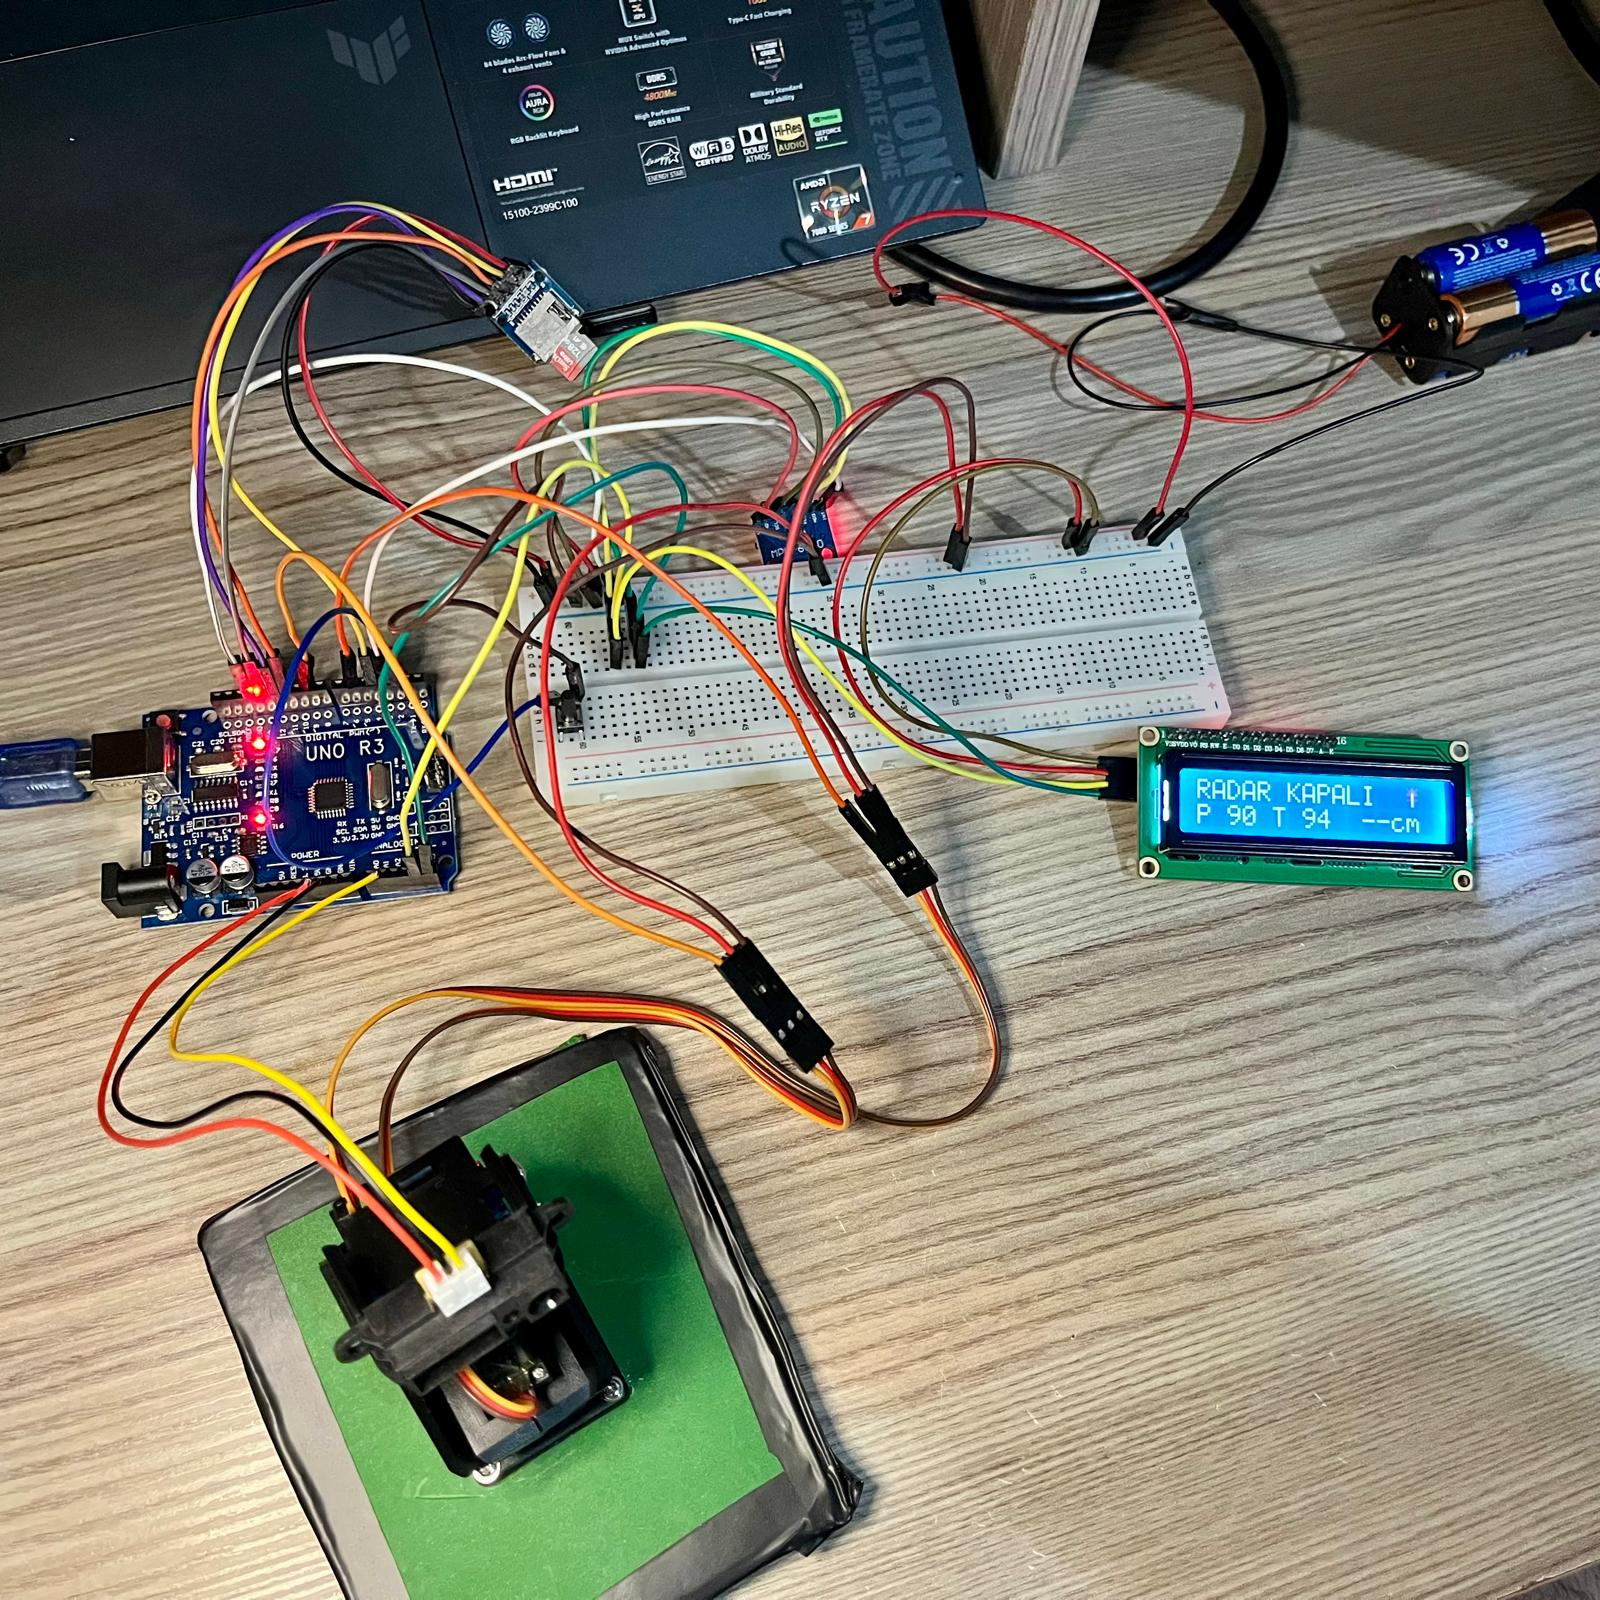
\includegraphics[width=0.82\textwidth]{tum_sistem_baglanti.jpeg}
    \caption{Sistemin genel bağlantı şeması ve prototip görünümü}
    \label{fig:tum_sistem}
\end{figure}

\subsection{Çalışmanın Amacı}
Projenin temel amacı, düşük maliyetli ve erişilebilir donanım bileşenleri ile iki eksenli tarama yapabilen, nesne algıladığında bunu kullanıcıya hem yerel hem de web tabanlı olarak bildirebilen bir radar simülasyon sistemi geliştirmektir. Bu amaç doğrultusunda sistemin yalnızca çalışması değil, aynı zamanda kararlı, izlenebilir ve raporlanabilir olması hedeflenmiştir.

Projenin alt hedefleri şu şekilde belirlenmiştir:
\begin{itemize}
    \item Sharp GP2Y0A02YK0F \cite{sharp_datasheet} kızılötesi mesafe sensörü ile 20--150~cm aralığında nesne tespiti gerçekleştirmek,
    \item MG90S ve SG90S servo motorlar aracılığıyla pan-tilt mekanizması üzerinde iki eksenli otomatik tarama hareketi sağlamak,
    \item 16x2 I2C LCD ekran üzerinden sistem durumu, hedef bilgisi ve mesafe bilgisini kullanıcıya göstermek,
    \item MPU6050 \cite{mpu6050_datasheet} ivmeölçer/jiroskop modülü ile platform hareketi ve titreşim bilgisini izlemek,
    \item SD kart modülü ile tarama verilerini kalıcı olarak kaydedilebilir hale getirmek,
    \item Web Serial API kullanarak tarayıcı tabanlı, gerçek zamanlı ve polar gösterimli bir radar arayüzü geliştirmek,
    \item Servo beslemesi, ortak topraklama, veri paketleme ve haberleşme kararlılığı gibi gömülü sistem problemlerine uygulanabilir çözümler üretmek.
\end{itemize}

\subsection{Çalışmanın Kapsamı}
Sistem; algılama, hareket, gömülü kontrol, yerel kullanıcı arayüzü, veri kaydı ve web tabanlı görselleştirme katmanlarından oluşmaktadır. Algılama katmanında Sharp IR sensörü analog mesafe verisi üretmektedir. Hareket katmanında pan ve tilt servo motorları, sensörün farklı açılara yönlendirilmesini sağlamaktadır. Gömülü kontrol katmanında Arduino Uno, sensör okuma, servo sürme, buton kontrolü, LCD güncelleme, MPU6050 okuma, SD karta yazma ve seri haberleşme görevlerini yürütmektedir.

Web katmanında ise Arduino'dan gelen JSON formatındaki telemetri paketleri tarayıcıda işlenmekte ve HTML5 Canvas üzerinde radar benzeri bir polar ekran oluşturulmaktadır. Bu yapı sayesinde kullanıcı, sistemin hedef algılama davranışını anlık olarak takip edebilmekte; pan açısı, tilt açısı, mesafe, hedef durumu, SD kart durumu, MPU6050 verileri ve Arduino besleme gerilimi gibi bilgileri aynı ekranda görebilmektedir.

\subsection{Çalışmanın Önemi}
Bu proje, gömülü sistem tasarımında tek bir bileşenin çalıştırılmasından daha ileri bir yaklaşım sunmaktadır. Servo motorların ani akım ihtiyacı, analog sensörlerin gürültülü yapısı, farklı haberleşme protokollerinin aynı mikrodenetleyici üzerinde birlikte kullanılması ve web arayüzü ile gerçek zamanlı veri aktarımı, gerçek mühendislik uygulamalarında karşılaşılan temel entegrasyon problemleridir. Bu nedenle çalışma, ders kapsamında geliştirilen bir prototip olmasına rağmen donanım-yazılım bütünleşmesi açısından uygulamalı bir deneyim sağlamaktadır.
